%!TEX TS-program = pdflatex
%  PHDTHESIS TEMPLATE FILE
%  Adopted from Thomas Fabricius and Henrik Aalborg Nielsen
%  Jan Larsen, IMM, DTU, Nov 2003 ver 1.0
%  Updated by Finn Kuno Christensen, fkc@imm.dtu.dk Aug 15, 2008

%  COMPILATION STEPS USING INVOLVING A PS FILE
% \documentclass[10pt,twoside,dvips]{book}
%  latex phdthesis.tex
%  dvips -D600 -Pamz -Pcmz -j0 phdthesis.dvi -o phdthesis.ps
%  ps2pdf -sPAPERSIZE=b5 phdthesis.ps phdthesis.pdf (or use Acrobat Distiller)

%  COMPILATION STEP USING PDFLATEX
\documentclass[10pt,twoside,pdftex]{book}
%  pdflatex phdthesis.tex

%%%%%%%%%%% MODIFY THESE LINES ONLY %%%%%%%%%%%%%%%%%%%%%%%%%%%%%%%%%%%%%%%%%%%%%%%%%%%%%%%%%
\def\thesisyear{2013} % Year thesis submitted
\def\thesisnumber{XX}  % Only number no year
\def\thesisauthor{Jenny Olsson} % Thesis author
\def\thesistitle{Timecritical network syncronization and signaling} % Title of thesis
\def\thesiskeywords{Network, Multicast, Synchronization, Timing, Rendering}
\def\thesisISBN{} %OBSOBS provide ISBN number for industrial phd students ONLY
%\def\thesisversion{print} %OBSOBS choose this for printed version send to printing
\def\thesisversion{net} %OBSOBS choose this for the net version for the web and publication database
%%%%%%%%%%%%%%%%%%%%%%%%%%%%%%%%%%%%%%%%%%%%%%%%%%%%%%%%%%%%%%%%%%%%%%%%%%%%%%%%%%%%%%%%%%%%%

\newcommand{\np}{$\mathcal{NP}$}

\usepackage[latin1]{inputenc}
\usepackage[english]{babel}
\usepackage{fancyheadings}
\usepackage{amsmath,amssymb,latexsym,epic,eepic,epsfig,graphics}
\usepackage{theorem}
\usepackage{immthesislayout}
\usepackage{graphicx}
\usepackage{placeins}
%\usepackage{listings}
%\usepackage{fontspec}
%\usepackage{minted}
%\usepackage[T1]{fontenc}
%\usepackage[scaled]{beramono}
%\setmonofont{Bitstream Vera Mono}
%\usepackage{eurosym}
\newcommand{\spacer}{
\begin{center}
* * *
\end{center}
}



\def\thesisISSN{0909-3192}
\def\ttitle{{\sf\textbf{\thesistitle}}}
\def\thesisdef{IMM-BSc-\thesisyear-\thesisnumber}
\usepackage{hyperref}
\def\printversion{print}
\ifx\thesisversion\printversion
  \special{papersize=176mm,250mm}
  \hypersetup{pdftitle={\thesistitle},
              pdfauthor={\thesisauthor},
              pdfsubject={\thesisdef},
              pdfkeywords={\thesiskeywords},
              breaklinks,
              bookmarksopen,
              bookmarksnumbered}
\else
  \hypersetup{pdftitle={\thesistitle},
              pdfauthor={\thesisauthor},
              pdfsubject={\thesisdef},
              pdfkeywords={\thesiskeywords},
              colorlinks,
              linkcolor=blue,
              breaklinks,
              bookmarksopen,
              bookmarksnumbered}
\fi

\newcommand{\papertitle}{}
\setcounter{tocdepth}{1} % 1 in final version 10 for debugging
\setcounter{secnumdepth}{3} % subsubsections get a number when this is 3

%\usepackage[T1]{fontenc}

%\usepackage[sc]{mathpazo}
%\linespread{1.05}         % Palatino needs more leading (space between lines)


\begin{document}

\thispagestyle{empty}
\vspace*{\fill}
\begin{center}
{\huge\ttitle}\\*[2.5cm]
\Large\sf\thesisauthor\\*[4.5cm]
\small\sf Stockholm \thesisyear\\
{\sf KTH}\\
\end{center}
\vspace*{\fill}
%\newpage
%\thispagestyle{empty}
%\vspace*{11cm}
%\\



% PREFACE CHAPTERS INCLUDE

\mbox{}
\vspace{3cm}
\begin{center}
\begin{minipage}[center]{0.80\textwidth}

\begin{center}
{\normalsize \textbf{Abstract.}}
\end{center}
This bachelor thesis is about synchronizing rendering over an network. Since projectors have a limited resolution several projectors needs to be used to get a specific high resolution. If these projectors are connected to different computers the rendering needs to be synchronized. 

add stuff on how i did this
\end{minipage}
\end{center}



\frontmatter
\pagenumbering{roman}


\chapter{Summary}

This thesis was written in the spring of 2013. It is an investigation into different solutions on how to sychronize rendering, on different computers, over an network. A possible use case is to manage projections that needs to combine a number of projectors to achieve a desired resolution, since projectors have a limited resolution. 

Different solutions on how to achieve synchronizations has been investigated, starting with the solution implemented in the NTP-protocol. 

\markboth{}{}
\chapter{Resum\'e} %{(Summary in Swedish?)}




\markboth{}{}
\chapter{Preface}

This thesis was written at 23c in Stockholm as the completion of my bachelors degree in Computer Engineering from The Royal Institute of Technology in Kista. It was started in March of 2013 and consists of 15 ECTS points. 

It presents a possible solution on how to synchronize the rendering processes on different computers over a network. 

This thesis and the code presented has been written by me and in the cases where other sources has been used this is clearly cited. 


\vspace{20mm}
\mbox{}\hfill
\begin{minipage}[t]{80mm}
  Stockholm 2013\\
  \vspace{1cm}\\
  Jenny Olsson
\end{minipage}

\subsection*{Glossary}

\subsubsection*{NTP}
Network Time Protocol, used to synchronize computer clocks over a network. 

\subsubsection*{Frameskipping}
Skipping forward a certain number of frames in an animation.

\subsubsection*{Tweening}
Also known as inbetweening. Technique for creating linear animations by defining the start and the end states of the animation. 

\subsubsection*{Timestep}
Defining the amount of time between two steps in the animation, making the animation depend on time rather than framerate.

\subsubsection*{Round trip delay}
The delay in time between sending a message and recieving a reply. 

\markboth{}{}
\chapter{Acknowledgements}

I would like to thank 23 Critters, especially Mathias Tervo and Kristoffer Smedlund, for presenting me with the problem and having great patiece in discusing it with me. 

% I suppose there will be a lot of people to thank for this.

Finally i would like to thank Sanna Barsk for the extensive proof-reading of this thesis. 


\markboth{}{}

% TABLE OF CONTENTS
\newpage\mbox{}\newpage
\chaptermark{Contents}
\renewcommand{\sectionmark}[1]{\markright{#1}}
\sectionmark{Contents}
\addtolength{\parskip}{-\baselineskip}
\tableofcontents
\addtolength{\parskip}{\baselineskip}
\renewcommand{\sectionmark}[1]{\markright{\thesection\ #1}}


% MAIN CHAPTERS INCLUDE
\mainmatter

\chapter{About synchronization}

\begin{quotation}
\bf You may delay, but time will not.
\rm \center \em - Benjamin Franklin
\end{quotation}

\section{Background}

Because projectors and screens have a limited resolution, achieving a specific higher resolution requires combining several screens or projectors. This leads to a need to synchronize the graphics-rendering of an arbitrary number of computers, connected to these screens or projectors. This thesis will explore the possibility of synchronizing rendering.

The work of this thesis will ultimately be used in a system to synchronize the rendering in a platform for graphics visualisation written in C++, OpenGL3 and GLSL. According to the specification, specific events also needs to be able to be sent to the clients, and the clients should perform specific animations on recieving these events.  

\subsection{When is the rendering synchronized?}

Research has been made into the maximum amount of delay acceptable for the human eye between Audio and Video\footnote{\url{http://tech.ebu.ch/docs/r/r037.pdf}, EBU}, as this is important in the broadcasting of television. No research into what could be ''acceptable'' asychronization for the human eye in video to video synchronization will be made in this thesis, it will be assumed that it is a soft Real Time system and that the delay between the video should be as short as possible, an best effort system. For the sake of clarity we discuss delays in milliseconds.

\subsection{What needs to be synchronized?}

Since the clients rendering the animations will be distributed on different computers it cannot be assumed that the clocks on these computers are in sync with each other, this needs to be solved, the clients needs to have the same perception of time. When recieving a message from the server, all clients needs to synchronize their animations with each other, thus the clients needs to have some kind of concept of their, or the other clients latencies. 

\subsection{What is specific for synchronizing rendering?}
There are a few tools available when working with rendering, there is first of all the possibility to change the speed and start time of animations but also the possibility to frameskip. There is also the possibility to framestep. 

\section{Synchronizing clocks over an network}
The problem of synchronizing computer clocks over an network has been investigated since the early days of networks. There are a few well known algoritms, these are the ones looked into in the making of this thesis. 
\subsection{The NTP algorithm}
\label{sec:ntp}

The NTP protocol\cite{mills} was originally devlopeded in 1985 by David L.Mills. It is used to synchronize clocks over a network by calculating the master offset using the round trip delay. NTP is still in use today, the latest RTC is from June 2010\footnote{\url{https://tools.ietf.org/html/rfc5905}}.

The NTP algorithm uses four different timestamps to calculate the round trip delay. 

\begin{itemize}
  \item[] \textbf{t0} is the time of the request packet transmission
  \item[] \textbf{t1} is the time of the request packet reception
  \item[] \textbf{t2} is the time of the response packet transmission
  \item[] \textbf{t3} is the time of the response packet reception.
\end{itemize}
\label{fig:ntpvars}

The timestamps of t0 and t3 is set by the sender and t1 and t2 by the reciever. The sender then calculates the round trip delay, $\delta$. 

\begin{displaymath}
	\delta = (\text{t3} - \text{t0}) - (\text{t2} - \text{t1})
\end{displaymath}
\label{fig:ntpdelta}

NTP assumes that the delay of the sender and the reciever is equal, and thus calculates the master offset, $\theta$,  as below. 

\begin{displaymath}
	\theta = \frac{(\text{t3} - \text{t0}) - (\text{t2} - \text{t1})}{2}
\end{displaymath}
\label{fig:ntpmo}


\subsection{The Berkley algorithm}
The Berkley algorithm was written by Gusella and Zatti in 1989. A simplification of the steps of the algorithm is shown below. 

\begin{enumerate}
\item A master polls slaves, the slaves reply with their time.
\item The master uses the round-trip time of the messages to estimate the time of each slave and the master's own time.
\item The master calculates an average of the clock times, ignoring extreme values.
\item The master sends the slaves their delta, which can be positive or negative. 
\end{enumerate}
\label{fig:mifare-auth}

The delta value is used by each slave to adapt their time to the choosen master time. 

%needs references

\subsection{Cristians algorithm}
\label{sec:christian}
Cristians algorithm\cite{cristian}, developed in 1989 by Flaviu Cristian, is used for synchronizing clocks by calculating the round trip time. It is a probabilistic algorithm\cite{cristian}, meaning that it it delivers a better accuracy the shorter the round trip delay time is. 

The algorithm works as follows. The server sends a message to the client, and the client replies. When the server recieves the reply from the client it calculates the round trip delay time, that is, the time passed between sending the request from the server and recieving the reply from the client divided by 2. This assumes that the latency of the server and the client is equal.

The server then sends the sum of its own time added with the round trip delay time to the client, and the client sets this as its own time. 

\begin{figure}[h!]
	\begin{displaymath}
		\text{Client time} = \text{Server time} + \text{Round trip delay time}
	\end{displaymath}
	\caption{Setting the time on the Client}
	\label{fig:crist}
\end{figure}


\subsection{PTP and GPS}

The Precision Time Protocol, abbriviates PTP, is a protocol used for high accuracy synchronization in time critical systems. The first RTC is from 2002. Although PTP achieves a very high level of synchronization it was believed in the making of this thesis that synchronizing rendering would not require that kind of precision. 

One other solution for synchronizing the time of distributed applications is to use GPS. This has not been investigated further in this thesis since this would require that all clients had a GPS-sender/reciever, something that seemed improbable. 


\section{Problem definition}
\label{sec:problem_definition}

\begin{itemize}
  \item Can we synchronize the rendering on an arbitrary number of computers?
  \begin{itemize}
    \item How can we solve the messaging of synchronization-events?
  	\item When and how often do we need to synchronize?
    \item What techniques are available?
    \item Which way gives the tightest synchronization?
    \item Which way is the most efficient?
  	\item How can this be optimized?
  \end{itemize}
\end{itemize}
 % What ch 1 is about, explaining the problem, what synch is etc
\chapter{The Demo}

This section aims to explain the overall architecture and choices made for the demo, specific solutions for synchronization will be presented in the next chapter. 

All code is available at github: https://github.com/Rymdsnigel/thesis-demo

\section{Running the programs}
The demo program is written in python 2.7.2. It requires pygame 1.9.1, simplejson 2.1.6, docopt 0.6.1 and gevent 0.13.0. 

% How its started
% How to interact with the server

\section{Overall architecture}
The demo program consists of a server that continously accept connecting clients. 

\begin{figure}[h!]
\centering
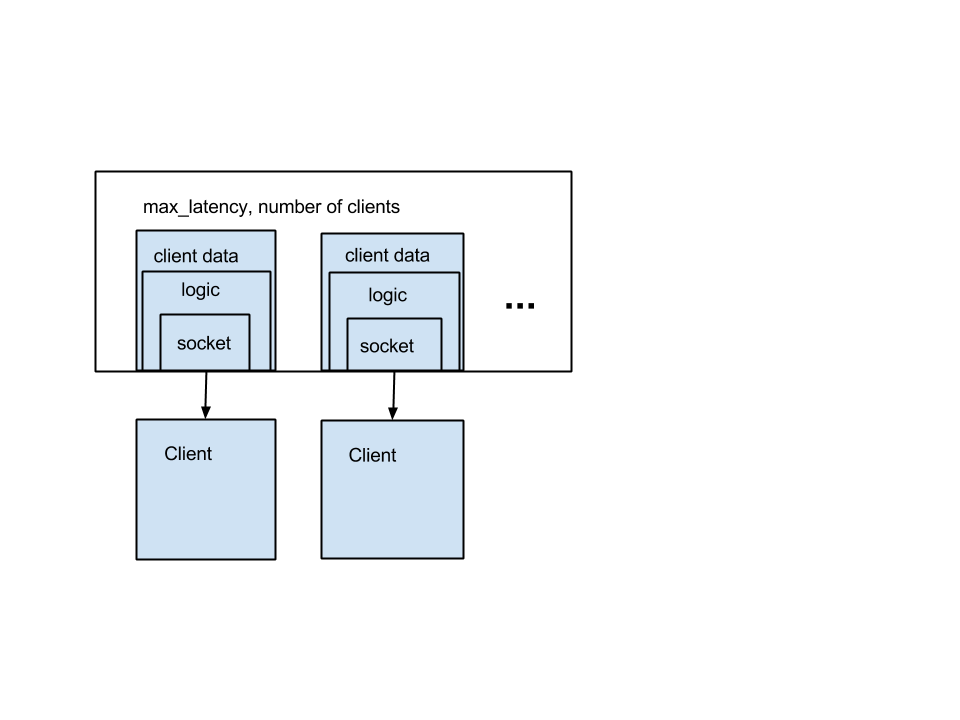
\includegraphics[width=1.0\textwidth]{figures/arch.png}
\caption{Overall architecture of the system.}
\end{figure}

\subsection{Why the Client-Server approach?}
Because there was a need to both generate and distribute specific events the client-server approach were chosen, rather than choosing a master among the clients, which might have been a more flexible choice if the generation of events had not been in the specification. The downside of this is that if the server should crash, the clients will loose their connection, the connection will not be reestablished by restarting the server.

\section{Design choises}

\section{Communication}

\subsection{Protocols}
The choice of TCP-sockets as opposed to UDP-sockets was made at an early stage of development. Although UDP is typically the ideal choice for time critical applications, customizing the needed control mechanisms would be outside the scope of this thesis. 

The choice of TCP presented proved to be problematic when it was discovered that TCP:s message buffering, using Nagels algoritm, generated a general delay in messaging, a delay of 20 ms both from the server as from the clients. This was discovered by measuring the delays of the application over localhost, where network delays should be close to 0. This issue also resulted in that more than one json object could be put on the queue of recieved events, which lead to a json-parsing error when trying to load the objects. These errors and the buffer delays were removed by disabling Nagels algorithm\footnote{\url{http://stackoverflow.com/questions/8617809/unstable-tcp-receive-times}} by setting the nodelay flag on the socket.

%source nagels algoritm

\begin{figure}[h!]
\centering
\texttt{self.s.setsockopt(socket.IPPROTO\_TCP, socket.TCP\_NODELAY, 1)}
\caption{Setting the nodelay flag on the socket}
\end{figure}

\subsection{Sockets}
The demo server communicates with the clients via gevent sockets since the sockets need to be threaded in order to not block the other processes. 

% ref to section about greenlets.
% explaining gevent sockets as opposed to regular sockets. 

\subsection{Replacing the networklayer}
Functional cohesion has been strived for, in order to make the part of the code pertaining to transport easily replaced by for example an implementation using UDP or implementation of a ready solution such as redis. Though this has not been entirely accomplished %in which ways is it not.






\subsection{Threading}
\label{sec:threading}

Both the server and the client has to achieve concurrency. This is achieved by letting both the TransportServers and the TransportClients inherit from gevent Greenlets %ref. 
Greenlets are in fact pseudothreads %ref
that share the same OS-thread so to release the control the threads must sleep on time critical operations to not block all other threads. 


\subsection{Messaging}
The server and clients sends and recieves json, the json is created using simplejson-library functions (dumps() and loads()), creating json from dicts. The functions for generating the dicts that will be the messages are specified in event.py. 

The choice of json for messaging, instead of using pickle or cpickle to read and write messages was made due to jsons speed of reading and writing \footnote{\url{http://kovshenin.com/2010/pickle-vs-json-which-is-faster/}, Kovshenin} and to support future flexibility in language since pickle and cpickle is python-specific. 

\subsection{Pygame}

Pygame, which is built on SDL(ref:http://www.pygame.org/wiki/about) was choosen for graphics due to its simplicity to work with. 



 % What ch 2 is about, architecture and design of demo program
\chapter{Running the demo application}

This section explains how the program works more specificly. It describes how to run it and how to interact with it. 

\section{Running the programs}
The demo program is written in python 2.7.2. It requires pygame 1.9.1, simplejson 2.1.6, docopt 0.6.1 and gevent 0.13.0. 

It is delivered with a bash-script named testrun\_2clients.sh that starts the server and two clients. The server and clients can also be started separately, but the server must be started first since the clients have no autodiscovery. 

The server requires no parameters and can be started as shown below. 

\begin{verbatim}
$ python server.py
there is no soundcard
\end{verbatim}

Starting the clients requires some flags to be specified. The --help flag displays the flags the client takes as arguments on startup. 

\begin{verbatim}
$ python client.py --help
Client rendering graphics

Usage:
  client.py [--port=<nr>]
            [--framerate=<frame/s>]
            [--x=<pixels>]
            [--y=<pixels>]
            [--pos <x1> <y1> <x2> <y2>]
  client.py (-h | --help)
  client.py --version

Options:
  -h --help     Show this screen.
  --version     Show version.
  --port=<nr>   Port number to bind to client [default: 5007].
  --framerate=<frame/s> Client framerate [default: 0].
  --x=<pixels> Width of client screen [default: 300].
  --y=<pixels> Height of client screen [default: 300].
  --pos <x1> <y1> <x2> <y2> Position of the part of the animation the client shows.
\end{verbatim}


\section{Emulating network delays}
In the beginning of the development the emulated network-delays were inserted using an gevent.sleep for a variable time in the code. This variable could be specified from command line. This was replaced by using netem \footnote{\url{http://www.linuxfoundation.org/collaborate/workgroups/networking/netem}}, a more flexible solution. 

With netem, delays can be bound to specific ports. The current version therefore requires the clients to be bound to specific ports in order to test them on ports with preset delays. The port to bind the client to must be specified when starting the client, using the --port flag. 

\begin{figure}[h! ]
\begin{verbatim}[]
tc qdisc add dev lo handle 1: root htb

tc class add dev lo parent 1: classid 1:1 htb rate 1000Mbps

tc class add dev lo parent 1:1 classid 1:11 htb rate 100Mbps
tc class add dev lo parent 1:1 classid 1:12 htb rate 100Mbps
tc class add dev lo parent 1:1 classid 1:13 htb rate 100Mbps

tc qdisc add dev lo parent 1:11 handle 10: netem delay 40ms
tc qdisc add dev lo parent 1:12 handle 20: netem delay 20ms
tc qdisc add dev lo parent 1:13 handle 30: netem delay 0ms

tc filter add dev lo protocol ip prio 1 u32 match ip dport 10001 0xffff flowid 1:11
tc filter add dev lo protocol ip prio 1 u32 match ip dport 10002 0xffff flowid 1:12
tc filter add dev lo protocol ip prio 1 u32 match ip dport 10003 0xffff flowid 1:13

tc filter add dev lo protocol ip prio 1 u32 match ip sport 10001 0xffff flowid 1:11
tc filter add dev lo protocol ip prio 1 u32 match ip sport 10002 0xffff flowid 1:12
tc filter add dev lo protocol ip prio 1 u32 match ip sport 10003 0xffff flowid 1:13
\end{verbatim}
\caption{Setting delays on port 10001, 10002 and 10003}
\end{figure}

\begin{figure}[h!]
\begin{verbatim}
tc qdisc del dev lo root
\end{verbatim}
\caption{Removing delays set on dev}
\end{figure}

\section{Interacting with the server}
%FIXME
The pygame window of the server captures the events. When clicked at it will display an animation that changes the color of a cube and changes it back. By holding down the right mouse button the cube can be moved. By pressing any keyboard key a sync event is sent from the server to all clients. 

\section{Communication}
The server continously accepts new connections but if the clients lose their connection to the server they will not automaticly reconnect. This means that if the server should crash, the clients lose their connection and the connection wont be reestablished by restarting the server.

 % What ch 3 is about, synchronizing the clients
%\chapter{Synchronizing the clients}

The synchronization of the animations has two major steps. First of all there is a continously running animation that takes input from the Tween class. This animation can be synchronized by giving every client a notion of how much delay there is between that client and a master, a master which could be the server.

The second step is to adapt the time the clients play specific parts of the animation when recieving a render event message from the server. An optimization of this is to frameskip the clients that are slower than a specified threshold.

\section{Synchronizing the time}

Because the clients may run on different computers the computer clock time cannot be used as a parameter to the animations since the computer clocks are unlikely to be in sync with each other. As shown in chapter 1 this is a well known problem in distributed systems, so the first step would be to implement one or several existing synchronization algorithms. 

A combination of the Berkley algoritm (ref section) and NTP (ref section) was used to synchronize the time of the clients and the server. Both NTP and the Berkley algorithm are designed to be used in intranets since they assume an evenly distributed delay. The end product that the work in this thesis is intended to be used in is assumed to run on an intranet. The accuracy given by these algoritms was assumed to be good enough. 

An artificial time is created both on the server and on the clients on start and this time never manipulated. Instead a delta value added to the artificial time is used as input to the animations.  

\subsection {Distributing deltas}

The server initiates the synchronization with the clients by sending a sync event message to the clients. The clients reply with the time they recieved the message, the time they send their reply and their old delta-value. The server then calculates each clients delta and sends each client a message containing their new delta. 

If the value of the old delta of the client and the new delta calculated by the server differs more than 2 milliseconds the server will send a new sync event as a message to the client, repeating the procedure until the delta is stable. 

Every time a new client connects to the server this client needs to synchronize its time with the server's. 

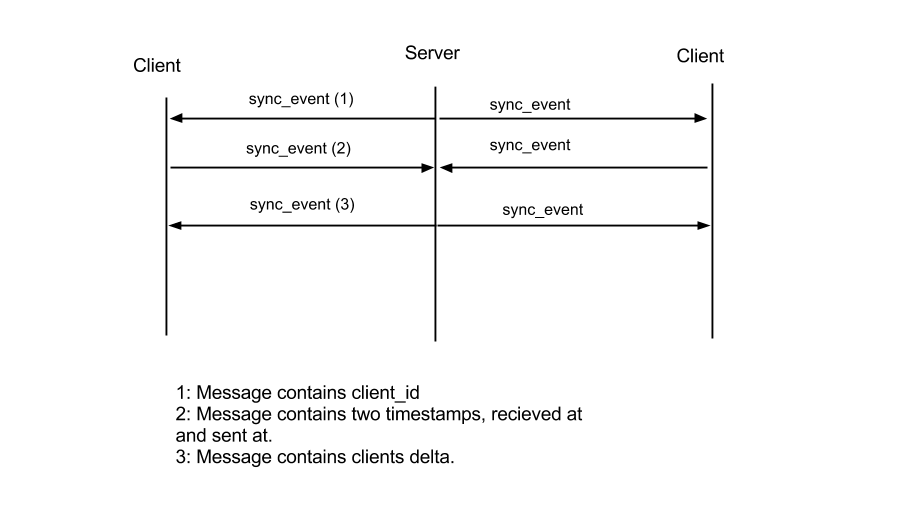
\includegraphics[width=1.0\textwidth]{figures/comm.png}

\subsection{Calculating deltas}
An implementation of NTP was used to calculate each clients latency, shown below.

\begin{verbatim}
self.delta = ((self.t_1 - self.t_0) + (self.t_2 - self.t_3))/2
\end{verbatim}

\subsection {Using the delta values}

All animations must take a timestamp as a parameter for playback. This is used to timestep through the animation. To create the timestamp the client uses the time acquired when the delta is added to its own local time. This way all client's animations will be synchronized, they will be at the same stage in the animation at the same time given that they have their correct delta value. 



\section{Distributing latencies}

\subsection{Finding the latency of a client}
The latency of each client is calculated by the server and sent to the client in an latency\_update\_event, along with the maximum latecy. The maximum latency is the latency of the client with the greatest latency. The client then calculates the wait period to sync to the client with the highest latency by subtracting its own latency from the maximum latency.

Client latencies are stored in an array on the server, everytime a client latency is updated the value of that respective row in the array is updated. The maximum latency is simply the largest number in this array.

Every time a new client connects to the server the server must send latency\_update\_events to all clients since the new connecting clients latency might be bigger than the current maximum latency. The maximum latency then needs to be redistributed to all clients. 

\begin{figure}[h!]
	\begin{displaymath}
		\text{applied\_latency} = \text{maximum\_latency} - \text{latency}
	\end{displaymath}
	\caption{Calculating the applied latency}
	\label{fig:applatency}
\end{figure} 

\subsection{Delaying animation start based on latency}
Before handling a new render event the client waits for the number of milliseconds specified by its applied latency. This way the faster clients will compensate for the slow ones. 

\subsection{Skipping frames if delay is to long}
If a clients latency is higher than a set threshold, the highest latency under the treshold is selected as the maximum latency and the client(s) above the threshold skip ahead instead. The clients that skip ahead will use their latency to skip that amount of time ahead in the animation. 



 % What ch 4 is about, possibly 
\chapter{Conclusion}
The goal of this thesis was to implent some kind of algoritm for synchronizing rendering on different computers over an network. 

Some important problems faced in development:
\begin{enumerate}
  \item Making sure that the client and the server agreed on a timestamp
  \item 
  \item 
\end{enumerate}



\subsection*{Outlook -- suggested improvements}
The demo is just an proof of concept.
 % Conclusions, suggested improvements


% APPENDIX CHAPTERS INCLUDE
\appendix

%\chapter{Log from two clients running on the same computer}
\begin{verbatim}
2013-05-09 22:59:00,340 - INFO - 1- Client animation started, time for animation: 200.0
2013-05-09 22:59:00,374 - INFO - 2- Client animation started, time for animation: 200.0
2013-05-09 22:59:00,540 - INFO - 1- Client animation started, time for animation: 200.0
2013-05-09 22:59:00,573 - INFO - 2- Client animation started, time for animation: 200.0
2013-05-09 22:59:01,115 - INFO - 1- Client animation started, time for animation: 200.0
2013-05-09 22:59:01,146 - INFO - 2- Client animation started, time for animation: 200.0
2013-05-09 22:59:01,320 - INFO - 1- Client animation started, time for animation: 200.0
2013-05-09 22:59:01,346 - INFO - 2- Client animation started, time for animation: 200.0
2013-05-09 22:59:01,956 - INFO - 1- Client animation started, time for animation: 200.0
2013-05-09 22:59:01,986 - INFO - 2- Client animation started, time for animation: 200.0
2013-05-09 22:59:02,156 - INFO - 1- Client animation started, time for animation: 200.0
2013-05-09 22:59:02,186 - INFO - 2- Client animation started, time for animation: 200.0
2013-05-09 22:59:02,741 - INFO - 1- Client animation started, time for animation: 200.0
2013-05-09 22:59:02,772 - INFO - 2- Client animation started, time for animation: 200.0
2013-05-09 22:59:02,941 - INFO - 1- Client animation started, time for animation: 200.0
2013-05-09 22:59:02,973 - INFO - 2- Client animation started, time for animation: 200.0
2013-05-09 22:59:03,784 - INFO - 1- Client animation started, time for animation: 200.0
2013-05-09 22:59:03,826 - INFO - 2- Client animation started, time for animation: 200.0
2013-05-09 22:59:03,984 - INFO - 1- Client animation started, time for animation: 200.0
2013-05-09 22:59:04,026 - INFO - 2- Client animation started, time for animation: 200.0
2013-05-09 22:59:05,120 - INFO - 1- Client animation started, time for animation: 200.0
2013-05-09 22:59:05,159 - INFO - 2- Client animation started, time for animation: 200.0
2013-05-09 22:59:05,321 - INFO - 1- Client animation started, time for animation: 200.0
2013-05-09 22:59:05,358 - INFO - 2- Client animation started, time for animation: 200.0
2013-05-09 22:59:05,932 - INFO - 1- Client animation started, time for animation: 200.0
2013-05-09 22:59:05,964 - INFO - 2- Client animation started, time for animation: 200.0
2013-05-09 22:59:06,132 - INFO - 1- Client animation started, time for animation: 200.0
2013-05-09 22:59:06,166 - INFO - 2- Client animation started, time for animation: 200.0
2013-05-09 22:59:11,041 - INFO - 1- Client applied latency: 29
2013-05-09 22:59:11,132 - INFO - 2- Client applied latency: 0
2013-05-09 22:59:12,464 - INFO - 1- Client applied latency: 30
2013-05-09 22:59:12,549 - INFO - 2- Client applied latency: 0
2013-05-09 22:59:13,751 - INFO - 1- Client applied latency: 29
2013-05-09 22:59:13,842 - INFO - 2- Client applied latency: 0
2013-05-09 22:59:15,048 - INFO - 1- Client applied latency: 29
2013-05-09 22:59:15,138 - INFO - 2- Client applied latency: 0
2013-05-09 22:59:16,771 - INFO - 1- Client animation started, time for animation: 200.0
2013-05-09 22:59:16,772 - INFO - 2- Client animation started, time for animation: 200.0
2013-05-09 22:59:16,971 - INFO - 2- Client animation started, time for animation: 200.0
2013-05-09 22:59:16,971 - INFO - 1- Client animation started, time for animation: 200.0
2013-05-09 22:59:17,614 - INFO - 1- Client animation started, time for animation: 200.0
2013-05-09 22:59:17,615 - INFO - 2- Client animation started, time for animation: 200.0
2013-05-09 22:59:17,814 - INFO - 1- Client animation started, time for animation: 200.0
2013-05-09 22:59:17,815 - INFO - 2- Client animation started, time for animation: 200.0
2013-05-09 22:59:18,431 - INFO - 1- Client animation started, time for animation: 200.0
2013-05-09 22:59:18,432 - INFO - 2- Client animation started, time for animation: 200.0
2013-05-09 22:59:18,631 - INFO - 1- Client animation started, time for animation: 200.0
2013-05-09 22:59:18,631 - INFO - 2- Client animation started, time for animation: 200.0
2013-05-09 22:59:19,271 - INFO - 2- Client animation started, time for animation: 200.0
2013-05-09 22:59:19,272 - INFO - 1- Client animation started, time for animation: 200.0
2013-05-09 22:59:19,471 - INFO - 2- Client animation started, time for animation: 200.0
2013-05-09 22:59:19,473 - INFO - 1- Client animation started, time for animation: 200.0
2013-05-09 22:59:20,176 - INFO - 1- Client animation started, time for animation: 200.0
2013-05-09 22:59:20,176 - INFO - 2- Client animation started, time for animation: 200.0
2013-05-09 22:59:20,375 - INFO - 2- Client animation started, time for animation: 200.0
2013-05-09 22:59:20,376 - INFO - 1- Client animation started, time for animation: 200.0
\end{verbatim}

\chapter{The Tween class}
\begin{verbatim}
class Tween(object):

    def __init__(self, *args, **kwargs):
        self.running = False
        self.logger = logging.getLogger('client')


    def play(self, start, end, time=1000.0, reverse=False,
interpolation=None,timestamp=None, skip=0):
        self.start = start
        self.end = end
        self.delta = end-start
        self.time = time
        self.timestep = self.delta /self.time
        self.value = start
        self.running = False
        self.reverse = reverse
        self.increasing = (end>start)
        self.running = True
        self.skip = skip
        self.timestamp = timestamp - skip  
		# this will result in frameskipping if skip is not 0
        self.logger.info("Client animation started, time for animation: 
			" + str(self.time))

    def step(self, current_time):
        if self.running :
            diff = current_time - self.timestamp
            self.value += diff * self.timestep
            if (self.value >= self.end) == self.increasing:
                if self.reverse:
                    self.play(self.value, self.start, timestamp=current_time,
time=self.time, reverse=False)
                else:
                    self.running = False
                    if self.value > self.end:
                        self.value = self.end
        self.timestamp = current_time

\end{verbatim}



\backmatter

\chaptermark{Bibliography}
\renewcommand{\sectionmark}[1]{\markright{#1}}
\sectionmark{Bibliography}

%%%%%%%BIBLIOGRAPHY INCLUDE%%%%%%%%%%%%%%%%%%%%%%%%%%%%%%%%%%%%%%%%%%%%%%

\bibliography{thesis}    % Bibliography
\bibliographystyle{plain}


\end{document}
